\documentclass{beamer}
\usetheme{Madrid}

\usepackage{amsmath, amssymb, amsthm}
\usepackage{graphicx}
\usepackage{gensymb}
\usepackage[utf8]{inputenc}
\usepackage{hyperref}
\usepackage{tikz}


\title{1.11.14 Matgeo}
\author{AI25BTECH11012 - Garige Unnathi}
\date{}

\begin{document}

\frame{\titlepage}

% Question frame
\begin{frame}
\frametitle{Question}
Find the equation of the conic, that satisfies the given conditions. \\ 
focus (-1,-2) and directrix x - 2y + 3 = 0.
\end{frame}


% Solution steps
\begin{frame}
\frametitle{Solution}
Let :
\begin{align}
    \textbf{F} = \begin{bmatrix}-1\\-2\end{bmatrix}\\
    directrix \quad equation \quad is : \begin{bmatrix}1\\-2\end{bmatrix}^{T}\textbf{x} = -3
\end{align}
The equation of a conic with directrix $\textbf{n}^{T}\textbf{x}$ = c , eccentricity e and focus \textbf{F} is given by:
\begin{align}
    g(\textbf{x}) = \textbf{x}^{T}\textbf{V}\textbf{x} + 2\textbf{u}^{T}\textbf{x} + f  = 0
\end{align}
\end{frame}

\begin{frame}
\frametitle{Solution}
where :

\begin{align*}
\textbf{V} = \lVert \textbf{n} \rVert^{2} \textbf{I} - e^{2}\textbf{n}\textbf{n}^{T} , \\
\textbf{u} = ce^{2}\textbf{n} - \lVert \textbf{n} \rVert^{2}\textbf{F} , \\
f = \lVert \textbf{n} \rVert^{2}\lVert \textbf{F} \rVert^{2} - c^{2}e^{2}
\end{align*}

\end{frame}

\begin{frame}
\frametitle{Solution}
From the question we can say that the conic is a parabola that is e = 1 ;\\
Calculating \textbf{V} ,\textbf{u} and f by using the above equations we get :
\begin{align}
   \textbf{V} = \begin{bmatrix}4 & 2\\2 & 1\end{bmatrix}\\
   \textbf{u} = \begin{bmatrix}2\\16\end{bmatrix}\\
   f = 16
\end{align}
\end{frame}



\begin{frame}
\frametitle{Solution}
Finding eigen values of $\textbf{V}$ :
\begin{align}
    det\lvert \textbf{V} - \lambda\textbf{I} \rvert = 0\\
    \begin{vmatrix} 4 - \lambda & 2 \\ 2 & 1 - \lambda \end{vmatrix} = 0\\
    \lambda^2 - 5\lambda = 0\\
    \lambda = 5 \quad and \quad 0 
\end{align}


\end{frame}

\begin{frame}
\frametitle{Solution}
Eigen vectors $\textbf{v}$ for any any square matrix $\textbf{A}$ is defined as :
\begin{align}
    \textbf{A}\textbf{v} = \lambda\textbf{v}\\
    (\textbf{A} - \lambda)\textbf{v} = 0 \\
    for \quad \lambda = 0 \quad v_1 = \begin{bmatrix}1\\-2\end{bmatrix}\\
        for \quad \lambda = 5 \quad v_2 = \begin{bmatrix}2\\1\end{bmatrix}
\end{align}

\end{frame}

\begin{frame}
\frametitle{Solution}
Substituting in the equation 0.3 we get :
\begin{align}
  \textbf{x}^{T}\begin{bmatrix}4 & 2\\2 & 1\end{bmatrix}\textbf{x} + 2\begin{bmatrix}2 \\ 16\end{bmatrix}^{T}\textbf{x} +16 =0
\end{align}
\end{frame}



% Graphical representation
\begin{frame}
\frametitle{Graphical Representation}
\begin{center}
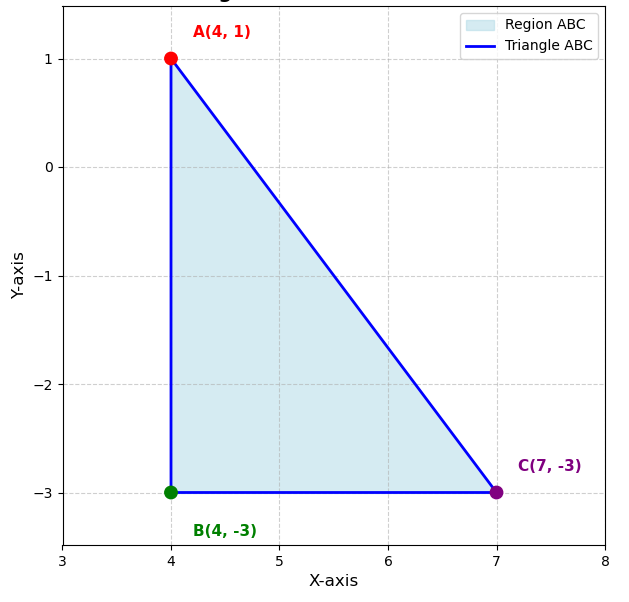
\includegraphics[width=0.6\linewidth]{/Users/unnathi/Documents/ee1030-2025/ai25btech11012/matgeo/8.2.48/figs/fig.png}
\end{center}
\end{frame}

\end{document}
